% Options for packages loaded elsewhere
\PassOptionsToPackage{unicode}{hyperref}
\PassOptionsToPackage{hyphens}{url}
%
\documentclass[
]{article}
\usepackage{amsmath,amssymb}
\usepackage{iftex}
\ifPDFTeX
  \usepackage[T1]{fontenc}
  \usepackage[utf8]{inputenc}
  \usepackage{textcomp} % provide euro and other symbols
\else % if luatex or xetex
  \usepackage{unicode-math} % this also loads fontspec
  \defaultfontfeatures{Scale=MatchLowercase}
  \defaultfontfeatures[\rmfamily]{Ligatures=TeX,Scale=1}
\fi
\usepackage{lmodern}
\ifPDFTeX\else
  % xetex/luatex font selection
\fi
% Use upquote if available, for straight quotes in verbatim environments
\IfFileExists{upquote.sty}{\usepackage{upquote}}{}
\IfFileExists{microtype.sty}{% use microtype if available
  \usepackage[]{microtype}
  \UseMicrotypeSet[protrusion]{basicmath} % disable protrusion for tt fonts
}{}
\makeatletter
\@ifundefined{KOMAClassName}{% if non-KOMA class
  \IfFileExists{parskip.sty}{%
    \usepackage{parskip}
  }{% else
    \setlength{\parindent}{0pt}
    \setlength{\parskip}{6pt plus 2pt minus 1pt}}
}{% if KOMA class
  \KOMAoptions{parskip=half}}
\makeatother
\usepackage{xcolor}
\usepackage[margin=1in]{geometry}
\usepackage{color}
\usepackage{fancyvrb}
\newcommand{\VerbBar}{|}
\newcommand{\VERB}{\Verb[commandchars=\\\{\}]}
\DefineVerbatimEnvironment{Highlighting}{Verbatim}{commandchars=\\\{\}}
% Add ',fontsize=\small' for more characters per line
\usepackage{framed}
\definecolor{shadecolor}{RGB}{248,248,248}
\newenvironment{Shaded}{\begin{snugshade}}{\end{snugshade}}
\newcommand{\AlertTok}[1]{\textcolor[rgb]{0.94,0.16,0.16}{#1}}
\newcommand{\AnnotationTok}[1]{\textcolor[rgb]{0.56,0.35,0.01}{\textbf{\textit{#1}}}}
\newcommand{\AttributeTok}[1]{\textcolor[rgb]{0.13,0.29,0.53}{#1}}
\newcommand{\BaseNTok}[1]{\textcolor[rgb]{0.00,0.00,0.81}{#1}}
\newcommand{\BuiltInTok}[1]{#1}
\newcommand{\CharTok}[1]{\textcolor[rgb]{0.31,0.60,0.02}{#1}}
\newcommand{\CommentTok}[1]{\textcolor[rgb]{0.56,0.35,0.01}{\textit{#1}}}
\newcommand{\CommentVarTok}[1]{\textcolor[rgb]{0.56,0.35,0.01}{\textbf{\textit{#1}}}}
\newcommand{\ConstantTok}[1]{\textcolor[rgb]{0.56,0.35,0.01}{#1}}
\newcommand{\ControlFlowTok}[1]{\textcolor[rgb]{0.13,0.29,0.53}{\textbf{#1}}}
\newcommand{\DataTypeTok}[1]{\textcolor[rgb]{0.13,0.29,0.53}{#1}}
\newcommand{\DecValTok}[1]{\textcolor[rgb]{0.00,0.00,0.81}{#1}}
\newcommand{\DocumentationTok}[1]{\textcolor[rgb]{0.56,0.35,0.01}{\textbf{\textit{#1}}}}
\newcommand{\ErrorTok}[1]{\textcolor[rgb]{0.64,0.00,0.00}{\textbf{#1}}}
\newcommand{\ExtensionTok}[1]{#1}
\newcommand{\FloatTok}[1]{\textcolor[rgb]{0.00,0.00,0.81}{#1}}
\newcommand{\FunctionTok}[1]{\textcolor[rgb]{0.13,0.29,0.53}{\textbf{#1}}}
\newcommand{\ImportTok}[1]{#1}
\newcommand{\InformationTok}[1]{\textcolor[rgb]{0.56,0.35,0.01}{\textbf{\textit{#1}}}}
\newcommand{\KeywordTok}[1]{\textcolor[rgb]{0.13,0.29,0.53}{\textbf{#1}}}
\newcommand{\NormalTok}[1]{#1}
\newcommand{\OperatorTok}[1]{\textcolor[rgb]{0.81,0.36,0.00}{\textbf{#1}}}
\newcommand{\OtherTok}[1]{\textcolor[rgb]{0.56,0.35,0.01}{#1}}
\newcommand{\PreprocessorTok}[1]{\textcolor[rgb]{0.56,0.35,0.01}{\textit{#1}}}
\newcommand{\RegionMarkerTok}[1]{#1}
\newcommand{\SpecialCharTok}[1]{\textcolor[rgb]{0.81,0.36,0.00}{\textbf{#1}}}
\newcommand{\SpecialStringTok}[1]{\textcolor[rgb]{0.31,0.60,0.02}{#1}}
\newcommand{\StringTok}[1]{\textcolor[rgb]{0.31,0.60,0.02}{#1}}
\newcommand{\VariableTok}[1]{\textcolor[rgb]{0.00,0.00,0.00}{#1}}
\newcommand{\VerbatimStringTok}[1]{\textcolor[rgb]{0.31,0.60,0.02}{#1}}
\newcommand{\WarningTok}[1]{\textcolor[rgb]{0.56,0.35,0.01}{\textbf{\textit{#1}}}}
\usepackage{graphicx}
\makeatletter
\def\maxwidth{\ifdim\Gin@nat@width>\linewidth\linewidth\else\Gin@nat@width\fi}
\def\maxheight{\ifdim\Gin@nat@height>\textheight\textheight\else\Gin@nat@height\fi}
\makeatother
% Scale images if necessary, so that they will not overflow the page
% margins by default, and it is still possible to overwrite the defaults
% using explicit options in \includegraphics[width, height, ...]{}
\setkeys{Gin}{width=\maxwidth,height=\maxheight,keepaspectratio}
% Set default figure placement to htbp
\makeatletter
\def\fps@figure{htbp}
\makeatother
\setlength{\emergencystretch}{3em} % prevent overfull lines
\providecommand{\tightlist}{%
  \setlength{\itemsep}{0pt}\setlength{\parskip}{0pt}}
\setcounter{secnumdepth}{-\maxdimen} % remove section numbering
\ifLuaTeX
  \usepackage{selnolig}  % disable illegal ligatures
\fi
\IfFileExists{bookmark.sty}{\usepackage{bookmark}}{\usepackage{hyperref}}
\IfFileExists{xurl.sty}{\usepackage{xurl}}{} % add URL line breaks if available
\urlstyle{same}
\hypersetup{
  pdftitle={3-state cSTM in R},
  pdfauthor={The DARTH workgroup},
  hidelinks,
  pdfcreator={LaTeX via pandoc}}

\title{3-state cSTM in R}
\usepackage{etoolbox}
\makeatletter
\providecommand{\subtitle}[1]{% add subtitle to \maketitle
  \apptocmd{\@title}{\par {\large #1 \par}}{}{}
}
\makeatother
\subtitle{With simulation-time dependency}
\author{The DARTH workgroup}
\date{}

\begin{document}
\maketitle

Developed by the Decision Analysis in R for Technologies in Health
(DARTH) workgroup: Fernando Alarid-Escudero, PhD (1) Eva A. Enns, MS,
PhD (2)\\
M.G. Myriam Hunink, MD, PhD (3,4) Hawre J. Jalal, MD, PhD (5) Eline
Krijkamp, PhD (6) Petros Pechlivanoglou, PhD (7,8) Alan Yang, MSc (8)

In collaboration of:

\begin{enumerate}
\def\labelenumi{\arabic{enumi}.}
\tightlist
\item
  Stanford University, Stanford, CA, USA
\item
  University of Minnesota School of Public Health, Minneapolis, MN, USA
\item
  Erasmus MC, Rotterdam, The Netherlands
\item
  Harvard T.H. Chan School of Public Health, Boston, USA
\item
  University of Ottawa, Ottawa, ON, Canada
\item
  Erasmus University, Rotterdam, The Netherlands
\item
  University of Toronto, Toronto ON, Canada
\item
  The Hospital for Sick Children, Toronto ON, Canada
\end{enumerate}

Please cite relevant publications when using this code:

\begin{itemize}
\item
  Alarid-Escudero, F., Krijkamp, E.M., Pechlivanoglou, P. et al.~A Need
  for Change! A Coding Framework for Improving Transparency in Decision
  Modeling. PharmacoEconomics 2019; 37.
  \url{https://doi.org/10.1007/s40273-019-00837-x}
\item
  Alarid-Escudero F, Krijkamp EM, Enns EA, Yang A, Hunink MGM
  Pechlivanoglou P, Jalal H. An Introductory Tutorial on Cohort
  State-Transition Models in R Using a Cost-Effectiveness Analysis
  Example. Medical Decision Making, 2023; 43(1). (Epub).
  \url{https://doi.org/10.1177/0272989X221103163}
\item
  Alarid-Escudero F, Krijkamp EM, Enns EA, Yang A, Hunink MGM
  Pechlivanoglou P, Jalal H. A Tutorial on Time-Dependent Cohort
  State-Transition Models in R using a Cost-Effectiveness Analysis
  Example. Medical Decision Making, 2023; 43(1).
  \url{https://doi.org/10.1177/0272989X221121747}
\item
  Krijkamp EM, Alarid-Escudero F, Enns EA, Jalal HJ, Hunink MGM,
  Pechlivanoglou P. Microsimulation modeling for health decision
  sciences using R: A tutorial. Medical Decision Making. 2018; 38(3).
  \url{https://journals.sagepub.com/doi/abs/10.1177/0272989X18754513}
\item
  Krijkamp EM, Alarid-Escudero F, Enns E, Pechlivanoglou P, Hunink MM,
  Jalal H. A Multidimensional Array Representation of State-Transition
  Model Dynamics. Medical Decision Making. 2020; 40(2).
  \url{https://doi.org/10.1177/0272989X19893973}
\item
  Jalal H, Pechlivanoglou P, Krijkamp E, Alarid-Escudero F, Enns E,
  Hunink MG. An Overview of R in Health Decision Sciences. Med Decis
  Making. 2017; 37(3).
  \url{https://journals.sagepub.com/doi/abs/10.1177/0272989X16686559}
\end{itemize}

\newpage

Change \texttt{eval} to \texttt{TRUE} if you want to knit this document.

\begin{Shaded}
\begin{Highlighting}[]
\FunctionTok{rm}\NormalTok{(}\AttributeTok{list =} \FunctionTok{ls}\NormalTok{())      }\CommentTok{\# clear memory (removes all the variables from the workspace)}
\end{Highlighting}
\end{Shaded}

\hypertarget{load-packages}{%
\section{01 Load packages}\label{load-packages}}

\begin{Shaded}
\begin{Highlighting}[]
\CommentTok{\# use this package to conveniently install other packages}
\ControlFlowTok{if}\NormalTok{ (}\SpecialCharTok{!}\FunctionTok{require}\NormalTok{(}\StringTok{\textquotesingle{}pacman\textquotesingle{}}\NormalTok{)) }\FunctionTok{install.packages}\NormalTok{(}\StringTok{\textquotesingle{}pacman\textquotesingle{}}\NormalTok{); }\FunctionTok{library}\NormalTok{(pacman) }

\CommentTok{\# load (install if required) packages from CRAN}
\FunctionTok{p\_load}\NormalTok{(}\StringTok{"devtools"}\NormalTok{,}\StringTok{"diagram"}\NormalTok{,}\StringTok{"dampack"}\NormalTok{)}
\end{Highlighting}
\end{Shaded}

\begin{verbatim}
## 
## The downloaded binary packages are in
##  /var/folders/sq/ys7t9cqj2wxf3br7m6sy6h_h0000gn/T//RtmpwByNcF/downloaded_packages
\end{verbatim}

\begin{Shaded}
\begin{Highlighting}[]
\CommentTok{\# load (install if required) packages from GitHub}
\CommentTok{\#install\_github("DARTH{-}git/darthtools", force = TRUE) \# Uncomment if there is a newer version}
\FunctionTok{p\_load\_gh}\NormalTok{(}\StringTok{"DARTH{-}git/darthtools"}\NormalTok{)}
\end{Highlighting}
\end{Shaded}

\hypertarget{load-functions}{%
\section{02 Load functions}\label{load-functions}}

\begin{Shaded}
\begin{Highlighting}[]
\CommentTok{\# all functions are in the darthtools package}
\end{Highlighting}
\end{Shaded}

\hypertarget{model-input}{%
\section{03 Model input}\label{model-input}}

\begin{Shaded}
\begin{Highlighting}[]
\DocumentationTok{\#\# General setup}
\NormalTok{cycle\_length    }\OtherTok{\textless{}{-}} \DecValTok{1}                             \CommentTok{\# cycle length equal to one year (use 1/12 for monthly)}
\NormalTok{n\_cycles        }\OtherTok{\textless{}{-}} \DecValTok{60}                            \CommentTok{\# number of cycles}
\NormalTok{v\_names\_cycles  }\OtherTok{\textless{}{-}} \FunctionTok{paste}\NormalTok{(}\StringTok{"cycle"}\NormalTok{, }\DecValTok{0}\SpecialCharTok{:}\NormalTok{n\_cycles)    }\CommentTok{\# cycle names}
\NormalTok{v\_names\_states  }\OtherTok{\textless{}{-}} \FunctionTok{c}\NormalTok{(}\StringTok{"H"}\NormalTok{, }\StringTok{"S"}\NormalTok{, }\StringTok{"D"}\NormalTok{)              }\CommentTok{\# state names}
\NormalTok{n\_states        }\OtherTok{\textless{}{-}} \FunctionTok{length}\NormalTok{(v\_names\_states)        }\CommentTok{\# number of health states }

\DocumentationTok{\#\#\# Discounting factors }
\NormalTok{d\_c }\OtherTok{\textless{}{-}} \FloatTok{0.03}        \CommentTok{\# annual discount rate for costs }
\NormalTok{d\_e }\OtherTok{\textless{}{-}} \FloatTok{0.03}        \CommentTok{\# annual discount rate for QALYs}

\DocumentationTok{\#\#\# Strategies }
\NormalTok{v\_names\_str     }\OtherTok{\textless{}{-}} \FunctionTok{c}\NormalTok{(}\StringTok{"Standard of Care"}\NormalTok{,         }\CommentTok{\# store the strategy names}
                     \StringTok{"Treatment A"}\NormalTok{, }
                     \StringTok{"Treatment B"}\NormalTok{)  }
\NormalTok{n\_str           }\OtherTok{\textless{}{-}} \FunctionTok{length}\NormalTok{(v\_names\_str)           }\CommentTok{\# number of strategies}

\DocumentationTok{\#\# Within{-}cycle correction (WCC) using Simpson\textquotesingle{}s 1/3 rule }
\NormalTok{v\_wcc }\OtherTok{\textless{}{-}} \FunctionTok{gen\_wcc}\NormalTok{(}\AttributeTok{n\_cycles =}\NormalTok{ n\_cycles,  }\AttributeTok{method =} \StringTok{"Simpson1/3"}\NormalTok{)}

\DocumentationTok{\#\#\# Transition intensity rates}
\NormalTok{r\_HS\_SoC  }\OtherTok{\textless{}{-}} \FloatTok{0.05}  \CommentTok{\# rate of becoming sick when healthy, under standard of care}
\NormalTok{r\_HS\_trtA }\OtherTok{\textless{}{-}} \FloatTok{0.04}  \CommentTok{\# rate of becoming sick when healthy, under treatment A}
\NormalTok{r\_HS\_trtB }\OtherTok{\textless{}{-}} \FloatTok{0.02}  \CommentTok{\# rate of becoming sick when healthy, under treatment B}
\NormalTok{r\_SD      }\OtherTok{\textless{}{-}} \FloatTok{0.1}   \CommentTok{\# rate of dying when sick}
\NormalTok{r\_base  }\OtherTok{\textless{}{-}} \FloatTok{0.003} \CommentTok{\# rate of dying when healthy at t = 0}
\NormalTok{rr\_annual  }\OtherTok{\textless{}{-}} \FloatTok{1.1}  \CommentTok{\# annual increase of mortality rate}
\CommentTok{\# rate of dying when healthy (time{-}dependent) {-} this is now a sequence of numbers}
\NormalTok{v\_r\_HD    }\OtherTok{\textless{}{-}}\NormalTok{ r\_base }\SpecialCharTok{*}\NormalTok{rr\_annual}\SpecialCharTok{\^{}}\NormalTok{(cycle\_length}\SpecialCharTok{*}\NormalTok{(}\DecValTok{0}\SpecialCharTok{:}\NormalTok{(n\_cycles}\DecValTok{{-}1}\NormalTok{)))}


\DocumentationTok{\#\#\#  Transition Probabilities}

\DocumentationTok{\#\#\# Converting rates to probabilities}
\CommentTok{\# p = 1 {-} exp( {-}r * cycle\_length)}
\NormalTok{p\_HS\_SoC  }\OtherTok{\textless{}{-}} \FunctionTok{rate\_to\_prob}\NormalTok{(}\AttributeTok{r =}\NormalTok{ r\_HS\_SoC, }\AttributeTok{t =}\NormalTok{ cycle\_length)  }\CommentTok{\# probability  of becoming sick when healthy, under SoC}
\NormalTok{p\_HS\_trtA }\OtherTok{\textless{}{-}} \FunctionTok{rate\_to\_prob}\NormalTok{(}\AttributeTok{r =}\NormalTok{ r\_HS\_trtA, }\AttributeTok{t =}\NormalTok{ cycle\_length) }\CommentTok{\# probability of becoming sick when healthy, under treatment A}
\NormalTok{p\_HS\_trtB }\OtherTok{\textless{}{-}} \FunctionTok{rate\_to\_prob}\NormalTok{(}\AttributeTok{r =}\NormalTok{ r\_HS\_trtB, }\AttributeTok{t =}\NormalTok{ cycle\_length) }\CommentTok{\# probability of becoming sick when healthy, under treatment B}
\NormalTok{p\_SD      }\OtherTok{\textless{}{-}} \FunctionTok{rate\_to\_prob}\NormalTok{(}\AttributeTok{r =}\NormalTok{ r\_SD, }\AttributeTok{t =}\NormalTok{ cycle\_length)      }\CommentTok{\# probability of dying when sick}
\NormalTok{v\_p\_HD    }\OtherTok{\textless{}{-}} \FunctionTok{rate\_to\_prob}\NormalTok{(}\AttributeTok{r =}\NormalTok{ v\_r\_HD, }\AttributeTok{t =}\NormalTok{ cycle\_length)    }\CommentTok{\# probability of dying when healthy (vector)}

\DocumentationTok{\#\#\# State rewards}
\DocumentationTok{\#\#\#\# Costs }
\NormalTok{c\_H       }\OtherTok{\textless{}{-}} \DecValTok{400}   \CommentTok{\# cost of one year in healthy state}
\NormalTok{c\_S       }\OtherTok{\textless{}{-}} \DecValTok{1000}  \CommentTok{\# cost of one year in sick state}
\NormalTok{c\_D       }\OtherTok{\textless{}{-}} \DecValTok{0}     \CommentTok{\# cost of one year in dead state}
\NormalTok{c\_trtA    }\OtherTok{\textless{}{-}} \DecValTok{800}   \CommentTok{\# cost of treatment A (per year) in healthy state}
\NormalTok{c\_trtB    }\OtherTok{\textless{}{-}} \DecValTok{1500}  \CommentTok{\# cost of treatment B (per year) in healthy state}
\DocumentationTok{\#\#\#\# Utilities}
\NormalTok{u\_H       }\OtherTok{\textless{}{-}} \DecValTok{1}     \CommentTok{\# utility when healthy }
\NormalTok{u\_S       }\OtherTok{\textless{}{-}} \FloatTok{0.5}   \CommentTok{\# utility when sick}
\NormalTok{u\_D       }\OtherTok{\textless{}{-}} \DecValTok{0}     \CommentTok{\# utility when dead}

\DocumentationTok{\#\#\# Discount weight for costs and effects }
\NormalTok{v\_dwc     }\OtherTok{\textless{}{-}} \DecValTok{1} \SpecialCharTok{/}\NormalTok{ ((}\DecValTok{1} \SpecialCharTok{+}\NormalTok{ (d\_e }\SpecialCharTok{*}\NormalTok{ cycle\_length)) }\SpecialCharTok{\^{}}\NormalTok{ (}\DecValTok{0}\SpecialCharTok{:}\NormalTok{n\_cycles))}
\NormalTok{v\_dwe     }\OtherTok{\textless{}{-}} \DecValTok{1} \SpecialCharTok{/}\NormalTok{ ((}\DecValTok{1} \SpecialCharTok{+}\NormalTok{ (d\_c }\SpecialCharTok{*}\NormalTok{ cycle\_length)) }\SpecialCharTok{\^{}}\NormalTok{ (}\DecValTok{0}\SpecialCharTok{:}\NormalTok{n\_cycles))}
\end{Highlighting}
\end{Shaded}

\hypertarget{construct-state-transition-models}{%
\section{04 Construct state-transition
models}\label{construct-state-transition-models}}

\begin{Shaded}
\begin{Highlighting}[]
\NormalTok{m\_P\_diag }\OtherTok{\textless{}{-}} \FunctionTok{matrix}\NormalTok{(}\DecValTok{0}\NormalTok{, }\AttributeTok{nrow =}\NormalTok{ n\_states, }\AttributeTok{ncol =}\NormalTok{ n\_states, }\AttributeTok{dimnames =} \FunctionTok{list}\NormalTok{(v\_names\_states, v\_names\_states))}
\NormalTok{m\_P\_diag[}\StringTok{"H"}\NormalTok{, }\StringTok{"H"}\NormalTok{ ] }\OtherTok{=} \StringTok{""}
\NormalTok{m\_P\_diag[}\StringTok{"H"}\NormalTok{, }\StringTok{"S"}\NormalTok{ ] }\OtherTok{=} \StringTok{""} 
\NormalTok{m\_P\_diag[}\StringTok{"H"}\NormalTok{, }\StringTok{"D"}\NormalTok{ ] }\OtherTok{=} \StringTok{""}
\NormalTok{m\_P\_diag[}\StringTok{"S"}\NormalTok{, }\StringTok{"S"}\NormalTok{ ] }\OtherTok{=} \StringTok{""}
\NormalTok{m\_P\_diag[}\StringTok{"S"}\NormalTok{, }\StringTok{"D"}\NormalTok{ ] }\OtherTok{=} \StringTok{""}
\NormalTok{m\_P\_diag[}\StringTok{"D"}\NormalTok{, }\StringTok{"D"}\NormalTok{ ] }\OtherTok{=} \StringTok{""}
\NormalTok{layout.fig }\OtherTok{\textless{}{-}} \FunctionTok{c}\NormalTok{(}\DecValTok{2}\NormalTok{, }\DecValTok{1}\NormalTok{)}
\FunctionTok{plotmat}\NormalTok{(}\FunctionTok{t}\NormalTok{(m\_P\_diag), }\FunctionTok{t}\NormalTok{(layout.fig), }\AttributeTok{self.cex =} \FloatTok{0.5}\NormalTok{, }\AttributeTok{curve =} \DecValTok{0}\NormalTok{, }\AttributeTok{arr.pos =} \FloatTok{0.8}\NormalTok{,  }
        \AttributeTok{latex =}\NormalTok{ T, }\AttributeTok{arr.type =} \StringTok{"curved"}\NormalTok{, }\AttributeTok{relsize =} \FloatTok{0.85}\NormalTok{, }\AttributeTok{box.prop =} \FloatTok{0.8}\NormalTok{, }
        \AttributeTok{cex =} \FloatTok{0.8}\NormalTok{, }\AttributeTok{box.cex =} \FloatTok{0.7}\NormalTok{, }\AttributeTok{lwd =} \DecValTok{1}\NormalTok{)}
\end{Highlighting}
\end{Shaded}

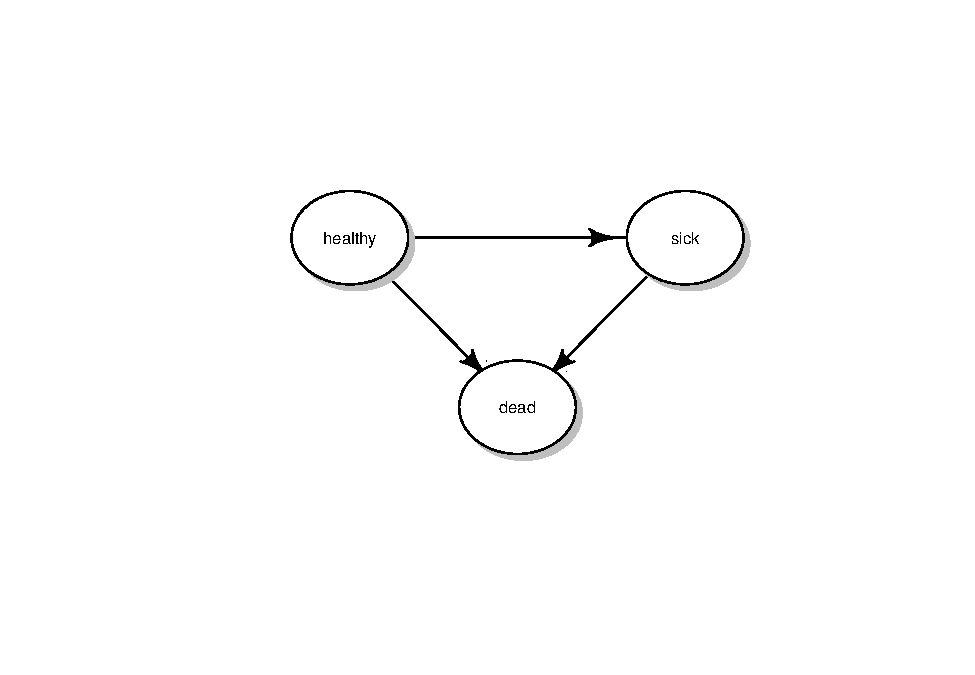
\includegraphics{cSTM_3state_time_files/figure-latex/unnamed-chunk-5-1.pdf}

\hypertarget{initial-state-vector}{%
\subsection{04.1 Initial state vector}\label{initial-state-vector}}

\begin{Shaded}
\begin{Highlighting}[]
\CommentTok{\# All starting healthy}
\NormalTok{v\_m\_init }\OtherTok{\textless{}{-}} \FunctionTok{c}\NormalTok{(}\StringTok{"H"} \OtherTok{=} \DecValTok{1}\NormalTok{, }\StringTok{"S"} \OtherTok{=} \DecValTok{0}\NormalTok{, }\StringTok{"D"} \OtherTok{=} \DecValTok{0}\NormalTok{)  }
\NormalTok{v\_m\_init}
\end{Highlighting}
\end{Shaded}

\begin{verbatim}
## H S D 
## 1 0 0
\end{verbatim}

\hypertarget{initialize-cohort-traces}{%
\subsection{04.2 Initialize cohort
traces}\label{initialize-cohort-traces}}

\begin{Shaded}
\begin{Highlighting}[]
\DocumentationTok{\#\#\# Initialize cohort trace for SoC }
\NormalTok{m\_M\_SoC }\OtherTok{\textless{}{-}} \FunctionTok{matrix}\NormalTok{(}\DecValTok{0}\NormalTok{, }
                  \AttributeTok{nrow =}\NormalTok{ (n\_cycles }\SpecialCharTok{+} \DecValTok{1}\NormalTok{), }\AttributeTok{ncol =}\NormalTok{ n\_states, }
                  \AttributeTok{dimnames =} \FunctionTok{list}\NormalTok{(v\_names\_cycles, v\_names\_states))}
\CommentTok{\# Store the initial state vector in the first row of the cohort trace}
\NormalTok{m\_M\_SoC[}\DecValTok{1}\NormalTok{, ] }\OtherTok{\textless{}{-}}\NormalTok{ v\_m\_init}

\DocumentationTok{\#\# Initialize cohort traces for treatments A and B}
\CommentTok{\# Structure and initial states are the same as for SoC}
\NormalTok{m\_M\_trtA }\OtherTok{\textless{}{-}}\NormalTok{ m\_M\_trtB }\OtherTok{\textless{}{-}}\NormalTok{ m\_M\_SoC}
\end{Highlighting}
\end{Shaded}

\hypertarget{create-transition-probability-arrays}{%
\subsection{04.3 Create transition probability
arrays}\label{create-transition-probability-arrays}}

\begin{Shaded}
\begin{Highlighting}[]
\DocumentationTok{\#\# Create transition probability arrays for strategy SoC }
\DocumentationTok{\#\#\# Initialize transition probability array for strategy SoC }
\CommentTok{\# All transitions to a non{-}death state are assumed to be conditional on survival}
\NormalTok{a\_P\_SoC }\OtherTok{\textless{}{-}} \FunctionTok{array}\NormalTok{(}\DecValTok{0}\NormalTok{,  }\CommentTok{\# Create 3{-}D array}
                \AttributeTok{dim =} \FunctionTok{c}\NormalTok{(n\_states, n\_states, n\_cycles),}
                \AttributeTok{dimnames =} \FunctionTok{list}\NormalTok{(v\_names\_states, v\_names\_states, }
\NormalTok{                                v\_names\_cycles[}\SpecialCharTok{{-}}\FunctionTok{length}\NormalTok{(v\_names\_cycles)])) }\CommentTok{\# name the dimensions of the array }

\DocumentationTok{\#\#\# Fill in array}
\DocumentationTok{\#\# Standard of Care}
\CommentTok{\# from Healthy}
\NormalTok{a\_P\_SoC[}\StringTok{"H"}\NormalTok{, }\StringTok{"H"}\NormalTok{, ] }\OtherTok{\textless{}{-}}\NormalTok{ (}\DecValTok{1} \SpecialCharTok{{-}}\NormalTok{ v\_p\_HD) }\SpecialCharTok{*}\NormalTok{ (}\DecValTok{1} \SpecialCharTok{{-}}\NormalTok{ p\_HS\_SoC)}
\NormalTok{a\_P\_SoC[}\StringTok{"H"}\NormalTok{, }\StringTok{"S"}\NormalTok{, ] }\OtherTok{\textless{}{-}}\NormalTok{ (}\DecValTok{1} \SpecialCharTok{{-}}\NormalTok{ v\_p\_HD) }\SpecialCharTok{*}\NormalTok{      p\_HS\_SoC}
\NormalTok{a\_P\_SoC[}\StringTok{"H"}\NormalTok{, }\StringTok{"D"}\NormalTok{, ] }\OtherTok{\textless{}{-}}\NormalTok{      v\_p\_HD}

\CommentTok{\# from Sick}
\NormalTok{a\_P\_SoC[}\StringTok{"S"}\NormalTok{, }\StringTok{"S"}\NormalTok{, ] }\OtherTok{\textless{}{-}} \DecValTok{1} \SpecialCharTok{{-}}\NormalTok{ p\_SD}
\NormalTok{a\_P\_SoC[}\StringTok{"S"}\NormalTok{, }\StringTok{"D"}\NormalTok{, ] }\OtherTok{\textless{}{-}}\NormalTok{     p\_SD}

\CommentTok{\# from Dead}
\NormalTok{a\_P\_SoC[}\StringTok{"D"}\NormalTok{, }\StringTok{"D"}\NormalTok{, ] }\OtherTok{\textless{}{-}} \DecValTok{1}

\DocumentationTok{\#\# Treatment A}
\NormalTok{a\_P\_trtA }\OtherTok{\textless{}{-}}\NormalTok{ a\_P\_SoC}
\NormalTok{a\_P\_trtA[}\StringTok{"H"}\NormalTok{, }\StringTok{"H"}\NormalTok{, ] }\OtherTok{\textless{}{-}}\NormalTok{ (}\DecValTok{1} \SpecialCharTok{{-}}\NormalTok{ v\_p\_HD) }\SpecialCharTok{*}\NormalTok{ (}\DecValTok{1} \SpecialCharTok{{-}}\NormalTok{ p\_HS\_trtA)}
\NormalTok{a\_P\_trtA[}\StringTok{"H"}\NormalTok{, }\StringTok{"S"}\NormalTok{, ] }\OtherTok{\textless{}{-}}\NormalTok{ (}\DecValTok{1} \SpecialCharTok{{-}}\NormalTok{ v\_p\_HD) }\SpecialCharTok{*}\NormalTok{      p\_HS\_trtA}

\DocumentationTok{\#\# Treatment B}
\NormalTok{a\_P\_trtB }\OtherTok{\textless{}{-}}\NormalTok{ a\_P\_SoC}
\NormalTok{a\_P\_trtB[}\StringTok{"H"}\NormalTok{, }\StringTok{"H"}\NormalTok{, ] }\OtherTok{\textless{}{-}}\NormalTok{ (}\DecValTok{1} \SpecialCharTok{{-}}\NormalTok{ v\_p\_HD) }\SpecialCharTok{*}\NormalTok{ (}\DecValTok{1} \SpecialCharTok{{-}}\NormalTok{ p\_HS\_trtB)}
\NormalTok{a\_P\_trtB[}\StringTok{"H"}\NormalTok{, }\StringTok{"S"}\NormalTok{, ] }\OtherTok{\textless{}{-}}\NormalTok{ (}\DecValTok{1} \SpecialCharTok{{-}}\NormalTok{ v\_p\_HD) }\SpecialCharTok{*}\NormalTok{      p\_HS\_trtB}

\DocumentationTok{\#\# Check if transition array and probabilities are valid}
\CommentTok{\# Check that transition probabilities are in [0, 1]}
\FunctionTok{check\_transition\_probability}\NormalTok{(a\_P\_SoC,  }\AttributeTok{verbose =} \ConstantTok{TRUE}\NormalTok{)}
\end{Highlighting}
\end{Shaded}

\begin{verbatim}
## [1] "Valid transition probabilities"
\end{verbatim}

\begin{Shaded}
\begin{Highlighting}[]
\FunctionTok{check\_transition\_probability}\NormalTok{(a\_P\_trtA, }\AttributeTok{verbose =} \ConstantTok{TRUE}\NormalTok{)}
\end{Highlighting}
\end{Shaded}

\begin{verbatim}
## [1] "Valid transition probabilities"
\end{verbatim}

\begin{Shaded}
\begin{Highlighting}[]
\FunctionTok{check\_transition\_probability}\NormalTok{(a\_P\_trtB, }\AttributeTok{verbose =} \ConstantTok{TRUE}\NormalTok{)}
\end{Highlighting}
\end{Shaded}

\begin{verbatim}
## [1] "Valid transition probabilities"
\end{verbatim}

\begin{Shaded}
\begin{Highlighting}[]
\CommentTok{\# Check that all rows sum to 1}
\FunctionTok{check\_sum\_of\_transition\_array}\NormalTok{(a\_P\_SoC,  }\AttributeTok{n\_states =}\NormalTok{ n\_states, }\AttributeTok{n\_cycles =}\NormalTok{ n\_cycles, }\AttributeTok{verbose =} \ConstantTok{TRUE}\NormalTok{)}
\end{Highlighting}
\end{Shaded}

\begin{verbatim}
## [1] "This is a valid transition array"
\end{verbatim}

\begin{Shaded}
\begin{Highlighting}[]
\FunctionTok{check\_sum\_of\_transition\_array}\NormalTok{(a\_P\_trtA, }\AttributeTok{n\_states =}\NormalTok{ n\_states, }\AttributeTok{n\_cycles =}\NormalTok{ n\_cycles, }\AttributeTok{verbose =} \ConstantTok{TRUE}\NormalTok{)}
\end{Highlighting}
\end{Shaded}

\begin{verbatim}
## [1] "This is a valid transition array"
\end{verbatim}

\begin{Shaded}
\begin{Highlighting}[]
\FunctionTok{check\_sum\_of\_transition\_array}\NormalTok{(a\_P\_trtB, }\AttributeTok{n\_states =}\NormalTok{ n\_states, }\AttributeTok{n\_cycles =}\NormalTok{ n\_cycles, }\AttributeTok{verbose =} \ConstantTok{TRUE}\NormalTok{)}
\end{Highlighting}
\end{Shaded}

\begin{verbatim}
## [1] "This is a valid transition array"
\end{verbatim}

\hypertarget{run-markov-model}{%
\section{05 Run Markov model}\label{run-markov-model}}

\begin{Shaded}
\begin{Highlighting}[]
\CommentTok{\# Iterative solution of age{-}dependent cSTM}
\ControlFlowTok{for}\NormalTok{(t }\ControlFlowTok{in} \DecValTok{1}\SpecialCharTok{:}\NormalTok{n\_cycles)\{}
  \DocumentationTok{\#\# Fill in cohort trace}
  \CommentTok{\# For SoC}
\NormalTok{  m\_M\_SoC[t }\SpecialCharTok{+} \DecValTok{1}\NormalTok{, ]  }\OtherTok{\textless{}{-}}\NormalTok{ m\_M\_SoC[t, ]  }\SpecialCharTok{\%*\%}\NormalTok{ a\_P\_SoC[, , t]}
  \CommentTok{\# For strategy A}
\NormalTok{  m\_M\_trtA[t }\SpecialCharTok{+} \DecValTok{1}\NormalTok{, ] }\OtherTok{\textless{}{-}}\NormalTok{ m\_M\_trtA[t, ] }\SpecialCharTok{\%*\%}\NormalTok{ a\_P\_trtA[, , t]}
  \CommentTok{\# For strategy B}
\NormalTok{  m\_M\_trtB[t }\SpecialCharTok{+} \DecValTok{1}\NormalTok{, ] }\OtherTok{\textless{}{-}}\NormalTok{ m\_M\_trtB[t, ] }\SpecialCharTok{\%*\%}\NormalTok{ a\_P\_trtB[, , t]}
\NormalTok{\}}

\DocumentationTok{\#\# Store the cohort traces in a list }
\NormalTok{l\_m\_M }\OtherTok{\textless{}{-}} \FunctionTok{list}\NormalTok{(}\AttributeTok{SoC =}\NormalTok{  m\_M\_SoC,}
              \AttributeTok{A   =}\NormalTok{  m\_M\_trtA,}
              \AttributeTok{B   =}\NormalTok{  m\_M\_trtB)}
\FunctionTok{names}\NormalTok{(l\_m\_M) }\OtherTok{\textless{}{-}}\NormalTok{ v\_names\_str}
\end{Highlighting}
\end{Shaded}

\hypertarget{plot-outputs}{%
\section{06 Plot Outputs}\label{plot-outputs}}

\hypertarget{plot-the-cohort-trace-for-strategies-soc}{%
\subsection{06.1 Plot the cohort trace for strategies
SoC}\label{plot-the-cohort-trace-for-strategies-soc}}

\begin{Shaded}
\begin{Highlighting}[]
\FunctionTok{plot\_trace}\NormalTok{(m\_M\_SoC) }
\end{Highlighting}
\end{Shaded}

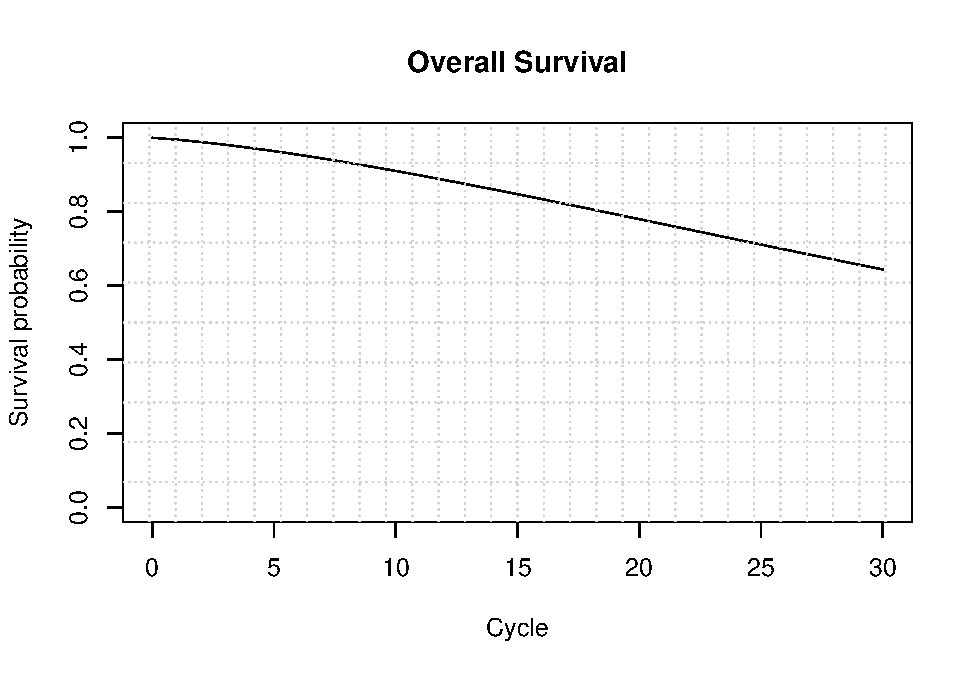
\includegraphics{cSTM_3state_time_files/figure-latex/unnamed-chunk-10-1.pdf}

\hypertarget{overall-survival-os}{%
\subsection{06.2 Overall Survival (OS)}\label{overall-survival-os}}

Print the overall survival for the Standard of Care

\begin{Shaded}
\begin{Highlighting}[]
\NormalTok{v\_os\_SoC }\OtherTok{\textless{}{-}} \DecValTok{1} \SpecialCharTok{{-}}\NormalTok{ m\_M\_SoC[, }\StringTok{"D"}\NormalTok{]    }\CommentTok{\# calculate the overall survival (OS) probability}
\NormalTok{v\_os\_SoC }\OtherTok{\textless{}{-}} \FunctionTok{rowSums}\NormalTok{(m\_M\_SoC[, }\DecValTok{1}\SpecialCharTok{:}\DecValTok{2}\NormalTok{])  }\CommentTok{\# alternative way of calculating the OS probability   }

\FunctionTok{plot}\NormalTok{(v\_os\_SoC, }\AttributeTok{type =} \StringTok{\textquotesingle{}l\textquotesingle{}}\NormalTok{, }
     \AttributeTok{ylim =} \FunctionTok{c}\NormalTok{(}\DecValTok{0}\NormalTok{, }\DecValTok{1}\NormalTok{),}
     \AttributeTok{ylab =} \StringTok{"Survival probability"}\NormalTok{,}
     \AttributeTok{xlab =} \StringTok{"Cycle"}\NormalTok{,}
     \AttributeTok{main =} \StringTok{"Overall Survival"}\NormalTok{)  }\CommentTok{\# create a simple plot showing the OS}

\CommentTok{\# add grid }
\FunctionTok{grid}\NormalTok{(}\AttributeTok{nx =}\NormalTok{ n\_cycles, }\AttributeTok{ny =} \DecValTok{10}\NormalTok{, }\AttributeTok{col =} \StringTok{"lightgray"}\NormalTok{, }\AttributeTok{lty =} \StringTok{"dotted"}\NormalTok{, }\AttributeTok{lwd =} \FunctionTok{par}\NormalTok{(}\StringTok{"lwd"}\NormalTok{), }
     \AttributeTok{equilogs =} \ConstantTok{TRUE}\NormalTok{) }
\end{Highlighting}
\end{Shaded}

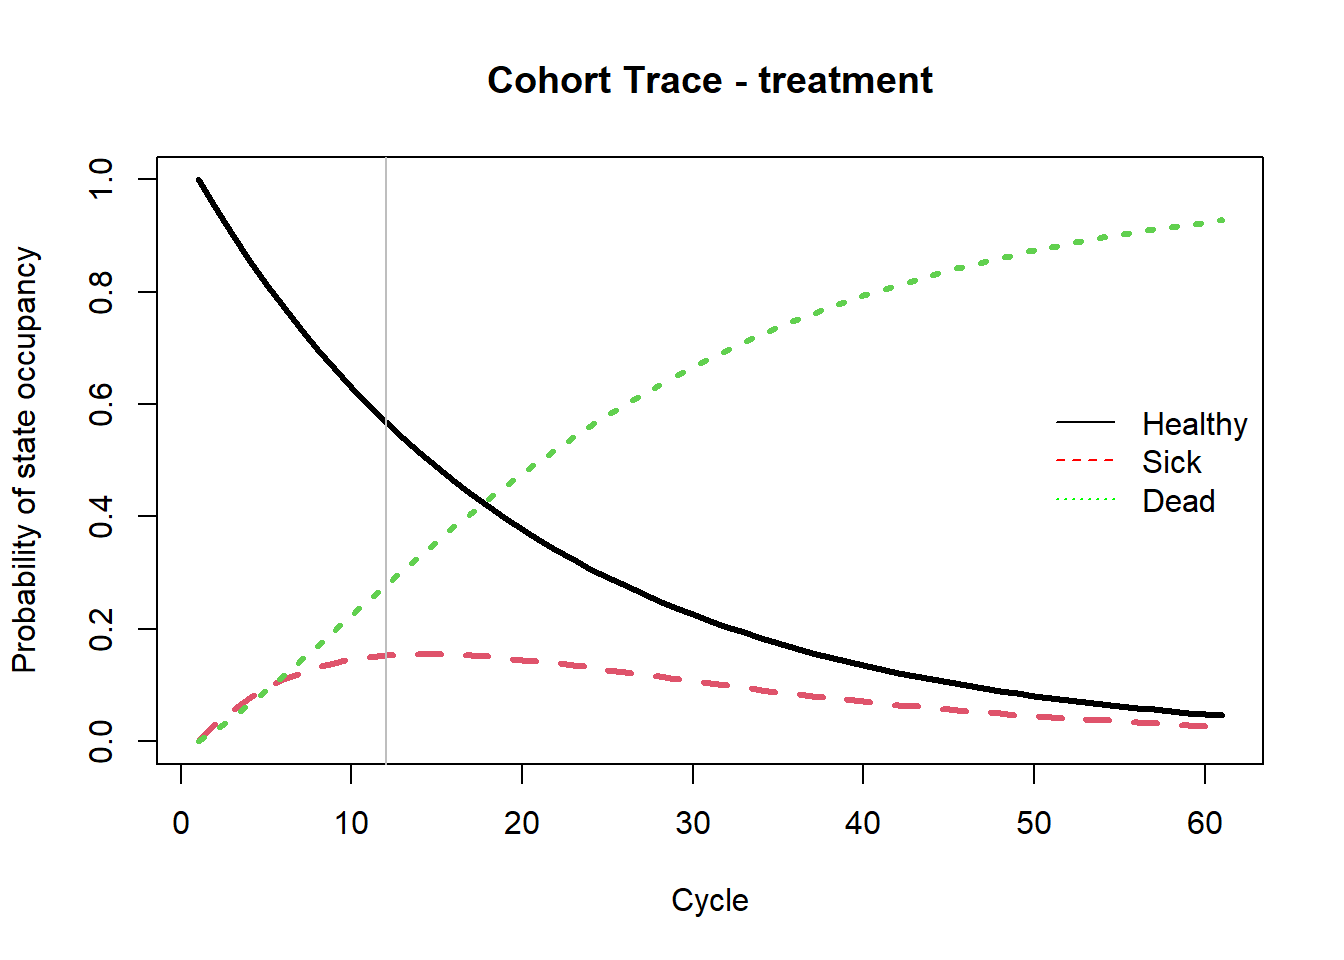
\includegraphics{cSTM_3state_time_files/figure-latex/unnamed-chunk-11-1.pdf}

\hypertarget{life-expectancy-le}{%
\subsection{06.2.1 Life Expectancy (LE)}\label{life-expectancy-le}}

\begin{Shaded}
\begin{Highlighting}[]
\NormalTok{le\_SoC }\OtherTok{\textless{}{-}} \FunctionTok{sum}\NormalTok{(v\_os\_SoC)  }\CommentTok{\# summing probability of OS over time  (i.e. life expectancy)}
\end{Highlighting}
\end{Shaded}

\hypertarget{disease-prevalence}{%
\subsection{06.2.2 Disease prevalence}\label{disease-prevalence}}

\begin{Shaded}
\begin{Highlighting}[]
\NormalTok{v\_prev }\OtherTok{\textless{}{-}}\NormalTok{ m\_M\_SoC[, }\StringTok{"S"}\NormalTok{]}\SpecialCharTok{/}\NormalTok{v\_os\_SoC}
\FunctionTok{plot}\NormalTok{(v\_prev,}
     \AttributeTok{ylim =} \FunctionTok{c}\NormalTok{(}\DecValTok{0}\NormalTok{, }\DecValTok{1}\NormalTok{),}
     \AttributeTok{ylab =} \StringTok{"Prevalence"}\NormalTok{,}
     \AttributeTok{xlab =} \StringTok{"Cycle"}\NormalTok{,}
     \AttributeTok{main =} \StringTok{"Disease prevalence"}\NormalTok{)}
\end{Highlighting}
\end{Shaded}

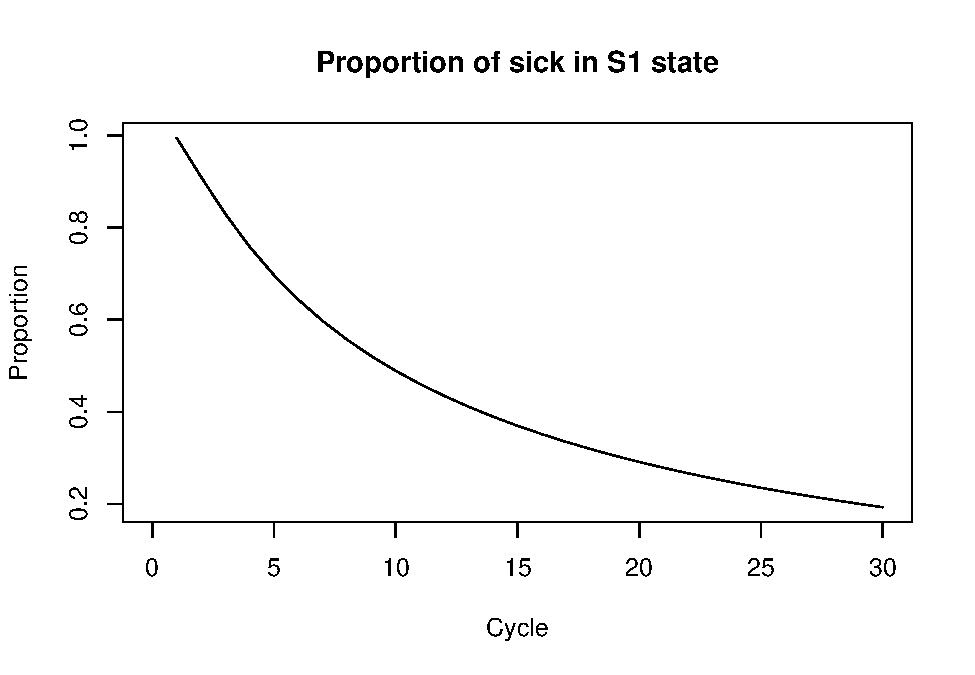
\includegraphics{cSTM_3state_time_files/figure-latex/unnamed-chunk-13-1.pdf}

\hypertarget{state-rewards}{%
\section{07 State Rewards}\label{state-rewards}}

\begin{Shaded}
\begin{Highlighting}[]
\DocumentationTok{\#\# Scale by the cycle length}

\CommentTok{\# Standard of Care}
\CommentTok{\# vector of state QALYs accrued each cycle}
\NormalTok{v\_u\_SoC    }\OtherTok{\textless{}{-}} \FunctionTok{c}\NormalTok{(}\AttributeTok{H  =}\NormalTok{ u\_H, }
                \AttributeTok{S  =}\NormalTok{ u\_S,}
                \AttributeTok{D  =}\NormalTok{ u\_D) }\SpecialCharTok{*}\NormalTok{ cycle\_length}
\CommentTok{\# vector of state costs accrued each cycle}
\NormalTok{v\_c\_SoC    }\OtherTok{\textless{}{-}} \FunctionTok{c}\NormalTok{(}\AttributeTok{H  =}\NormalTok{ c\_H, }
                \AttributeTok{S  =}\NormalTok{ c\_S,}
                \AttributeTok{D  =}\NormalTok{ c\_D) }\SpecialCharTok{*}\NormalTok{ cycle\_length}

\CommentTok{\# Treatment A}
\CommentTok{\# vector of state QALYs accrued each cycle}
\NormalTok{v\_u\_trtA   }\OtherTok{\textless{}{-}} \FunctionTok{c}\NormalTok{(}\AttributeTok{H  =}\NormalTok{ u\_H, }
                \AttributeTok{S  =}\NormalTok{ u\_S, }
                \AttributeTok{D  =}\NormalTok{ u\_D) }\SpecialCharTok{*}\NormalTok{ cycle\_length}
\CommentTok{\# vector of state costs accrued each cycle}
\NormalTok{v\_c\_trtA   }\OtherTok{\textless{}{-}} \FunctionTok{c}\NormalTok{(}\AttributeTok{H  =}\NormalTok{ c\_H }\SpecialCharTok{+}\NormalTok{ c\_trtA, }
                \AttributeTok{S  =}\NormalTok{ c\_S, }
                \AttributeTok{D  =}\NormalTok{ c\_D) }\SpecialCharTok{*}\NormalTok{ cycle\_length}

\CommentTok{\# Treatment B}
\CommentTok{\# vector of state QALYs accrued each cycle}
\NormalTok{v\_u\_trtB   }\OtherTok{\textless{}{-}} \FunctionTok{c}\NormalTok{(}\AttributeTok{H  =}\NormalTok{ u\_H, }
                \AttributeTok{S  =}\NormalTok{ u\_S, }
                \AttributeTok{D  =}\NormalTok{ u\_D) }\SpecialCharTok{*}\NormalTok{ cycle\_length}
\CommentTok{\# vector of state costs accrued each cycle}
\NormalTok{v\_c\_trtB   }\OtherTok{\textless{}{-}} \FunctionTok{c}\NormalTok{(}\AttributeTok{H  =}\NormalTok{ c\_H }\SpecialCharTok{+}\NormalTok{ c\_trtB, }
                \AttributeTok{S  =}\NormalTok{ c\_S, }
                \AttributeTok{D  =}\NormalTok{ c\_D) }\SpecialCharTok{*}\NormalTok{ cycle\_length}

\DocumentationTok{\#\# Store state rewards }
\CommentTok{\# Store the vectors of state utilities for each strategy in a list }
\NormalTok{l\_u   }\OtherTok{\textless{}{-}} \FunctionTok{list}\NormalTok{(}\AttributeTok{SoQ =}\NormalTok{ v\_u\_SoC,}
              \AttributeTok{A   =}\NormalTok{ v\_u\_trtA,}
              \AttributeTok{B   =}\NormalTok{ v\_u\_trtB)}
\CommentTok{\# Store the vectors of state cost for each strategy in a list }
\NormalTok{l\_c   }\OtherTok{\textless{}{-}} \FunctionTok{list}\NormalTok{(}\AttributeTok{SoQ =}\NormalTok{ v\_c\_SoC,}
              \AttributeTok{A   =}\NormalTok{ v\_c\_trtA,}
              \AttributeTok{B   =}\NormalTok{ v\_c\_trtB)}

\CommentTok{\# assign strategy names to matching items in the lists}
\FunctionTok{names}\NormalTok{(l\_u) }\OtherTok{\textless{}{-}} \FunctionTok{names}\NormalTok{(l\_c) }\OtherTok{\textless{}{-}}\NormalTok{ v\_names\_str}
\end{Highlighting}
\end{Shaded}

\hypertarget{compute-expected-outcomes}{%
\section{08 Compute expected outcomes}\label{compute-expected-outcomes}}

\begin{Shaded}
\begin{Highlighting}[]
\CommentTok{\# Create empty vectors to store total utilities and costs }
\NormalTok{v\_tot\_qaly }\OtherTok{\textless{}{-}}\NormalTok{ v\_tot\_cost }\OtherTok{\textless{}{-}} \FunctionTok{vector}\NormalTok{(}\AttributeTok{mode =} \StringTok{"numeric"}\NormalTok{, }\AttributeTok{length =}\NormalTok{ n\_str)}
\FunctionTok{names}\NormalTok{(v\_tot\_qaly) }\OtherTok{\textless{}{-}} \FunctionTok{names}\NormalTok{(v\_tot\_cost) }\OtherTok{\textless{}{-}}\NormalTok{ v\_names\_str}

\DocumentationTok{\#\# Loop through each strategy and calculate total utilities and costs }
\ControlFlowTok{for}\NormalTok{ (i }\ControlFlowTok{in} \DecValTok{1}\SpecialCharTok{:}\NormalTok{n\_str) \{}
\NormalTok{  v\_u\_str }\OtherTok{\textless{}{-}}\NormalTok{ l\_u[[i]]   }\CommentTok{\# select the vector of state utilities for the i{-}th strategy}
\NormalTok{  v\_c\_str }\OtherTok{\textless{}{-}}\NormalTok{ l\_c[[i]]   }\CommentTok{\# select the vector of state costs for the i{-}th strategy}
  
  \DocumentationTok{\#\#\# Expected QALYs and costs per cycle }
  \DocumentationTok{\#\# Vector of QALYs and Costs}
  \CommentTok{\# Apply state rewards }
\NormalTok{  v\_qaly\_str }\OtherTok{\textless{}{-}}\NormalTok{ l\_m\_M[[i]] }\SpecialCharTok{\%*\%}\NormalTok{ v\_u\_str }\CommentTok{\# sum the utilities of all states for each cycle}
\NormalTok{  v\_cost\_str }\OtherTok{\textless{}{-}}\NormalTok{ l\_m\_M[[i]] }\SpecialCharTok{\%*\%}\NormalTok{ v\_c\_str }\CommentTok{\# sum the costs of all states for each cycle}
  
  \DocumentationTok{\#\#\# Discounted total expected QALYs and Costs per strategy and apply within{-}cycle correction if applicable}
  \CommentTok{\# QALYs}
\NormalTok{  v\_tot\_qaly[i] }\OtherTok{\textless{}{-}} \FunctionTok{t}\NormalTok{(v\_qaly\_str) }\SpecialCharTok{\%*\%}\NormalTok{ (v\_dwe }\SpecialCharTok{*}\NormalTok{ v\_wcc)}
  \CommentTok{\# Costs}
\NormalTok{  v\_tot\_cost[i] }\OtherTok{\textless{}{-}} \FunctionTok{t}\NormalTok{(v\_cost\_str) }\SpecialCharTok{\%*\%}\NormalTok{ (v\_dwc }\SpecialCharTok{*}\NormalTok{ v\_wcc)}
\NormalTok{\}}
\end{Highlighting}
\end{Shaded}

\hypertarget{cost-effectiveness-analysis-cea}{%
\section{09 Cost-effectiveness analysis
(CEA)}\label{cost-effectiveness-analysis-cea}}

\begin{Shaded}
\begin{Highlighting}[]
\DocumentationTok{\#\# Incremental cost{-}effectiveness ratios (ICERs) }
\NormalTok{df\_cea }\OtherTok{\textless{}{-}} \FunctionTok{calculate\_icers}\NormalTok{(}\AttributeTok{cost       =}\NormalTok{ v\_tot\_cost, }
                          \AttributeTok{effect     =}\NormalTok{ v\_tot\_qaly,}
                          \AttributeTok{strategies =}\NormalTok{ v\_names\_str)}
\NormalTok{df\_cea}
\end{Highlighting}
\end{Shaded}

\begin{verbatim}
##                          Strategy      Cost   Effect Inc_Cost Inc_Effect
## Standard of Care Standard of Care  8696.761 12.90463       NA         NA
## Treatment B           Treatment B 30834.091 16.16428 22137.33   3.259648
## Treatment A           Treatment A 18138.224 13.81353       NA         NA
##                      ICER Status
## Standard of Care       NA     ND
## Treatment B      6791.325     ND
## Treatment A            NA     ED
\end{verbatim}

\begin{Shaded}
\begin{Highlighting}[]
\DocumentationTok{\#\# CEA table in proper format }
\NormalTok{table\_cea }\OtherTok{\textless{}{-}} \FunctionTok{format\_table\_cea}\NormalTok{(df\_cea) }
\NormalTok{table\_cea}
\end{Highlighting}
\end{Shaded}

\begin{verbatim}
##                          Strategy Costs ($) QALYs Incremental Costs ($)
## Standard of Care Standard of Care     8,697 12.90                  <NA>
## Treatment B           Treatment B    30,834 16.16                22,137
## Treatment A           Treatment A    18,138 13.81                  <NA>
##                  Incremental QALYs ICER ($/QALY) Status
## Standard of Care                NA          <NA>     ND
## Treatment B                   3.26         6,791     ND
## Treatment A                     NA          <NA>     ED
\end{verbatim}

\begin{Shaded}
\begin{Highlighting}[]
\DocumentationTok{\#\# CEA frontier }
\FunctionTok{plot}\NormalTok{(df\_cea, }\AttributeTok{label =} \StringTok{"all"}\NormalTok{, }\AttributeTok{txtsize =} \DecValTok{14}\NormalTok{) }\SpecialCharTok{+}
  \FunctionTok{expand\_limits}\NormalTok{(}\AttributeTok{x =} \FunctionTok{max}\NormalTok{(table\_cea}\SpecialCharTok{$}\NormalTok{QALYs) }\SpecialCharTok{+} \FloatTok{0.1}\NormalTok{) }\SpecialCharTok{+}
  \FunctionTok{theme}\NormalTok{(}\AttributeTok{legend.position =} \FunctionTok{c}\NormalTok{(}\FloatTok{0.8}\NormalTok{, }\FloatTok{0.3}\NormalTok{))}
\end{Highlighting}
\end{Shaded}

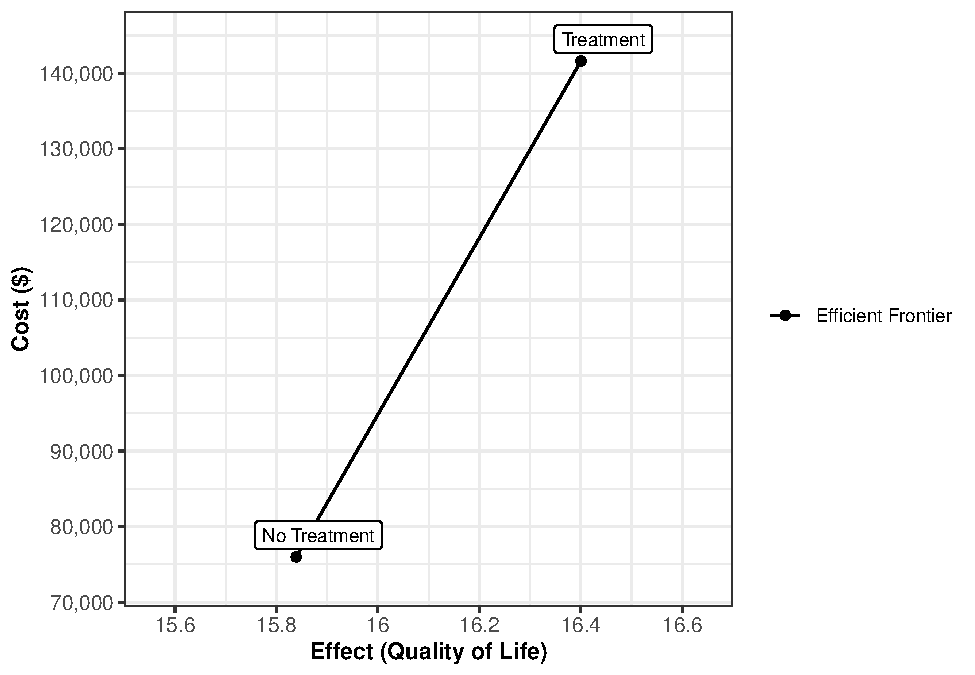
\includegraphics{cSTM_3state_time_files/figure-latex/unnamed-chunk-18-1.pdf}

\end{document}
